%*----------- SLIDE -------------------------------------------------------------
\begin{frame}[c]{Methodology}
  %\transboxin[duration=1,direction=30]
  The methods adopted for the development of this project were divided into three parts: theoretical foundation, development, and results. \linebreak
  \transboxin[duration=1,direction=30]

  \centering
  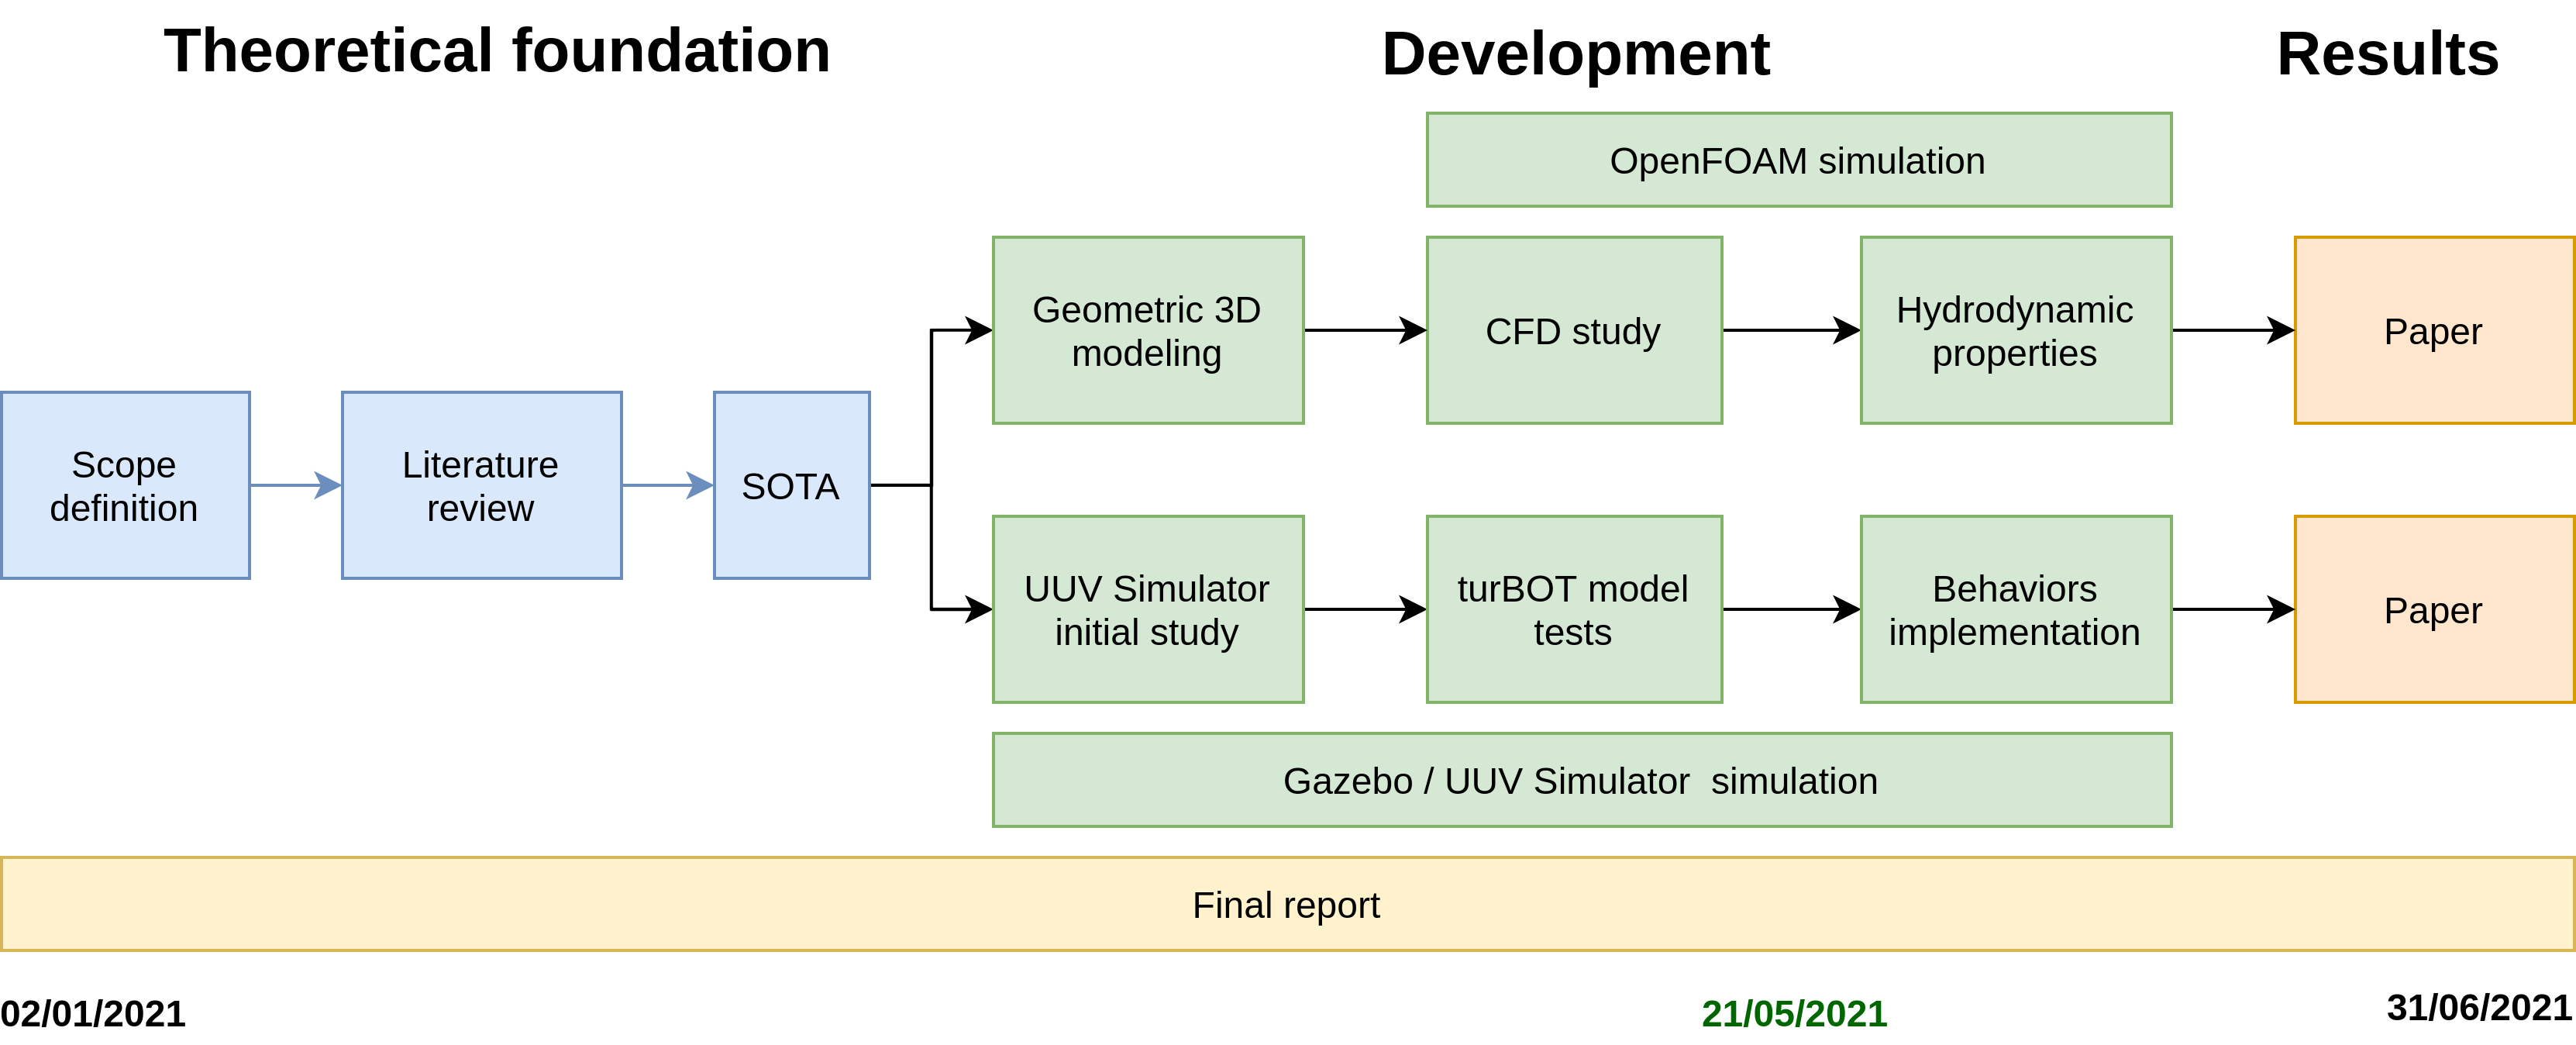
\includegraphics[width=.9\textwidth]{metodo.png}
\end{frame}
%-
%*----------- SLIDE -------------------------------------------------------------
\begin{frame}[t]{Vehicle's design}
  \transboxout[duration=0.5]
  \begin{columns}
    \column{.0\textwidth}
    \column{.3\textwidth}
      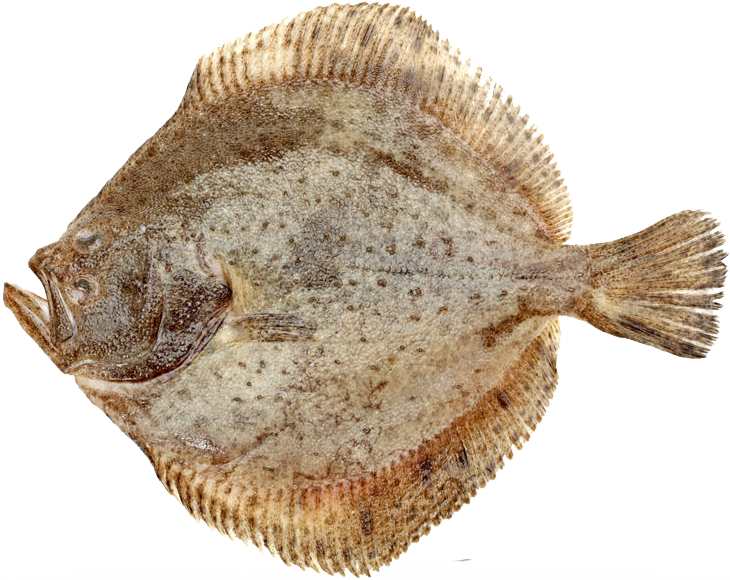
\includegraphics[width=.85\textwidth]{turbotreal.png}
      \linebreak
      \linebreak
      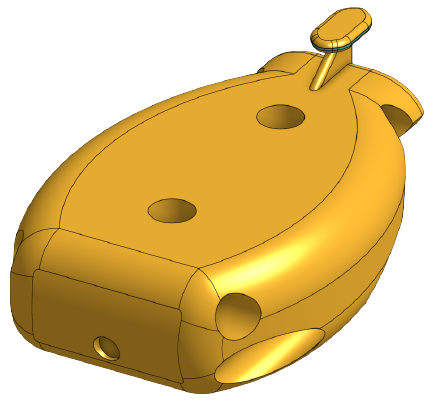
\includegraphics[width=.8\textwidth]{turbot_design.png}
    \column{.7\textwidth}
      The first vehicle's design was made using OnShape software,based on real-life Turbot Fish.  
      \linebreak
      \linebreak
      After CFD analysis, an optimized design a will be developed by the team.
  \end{columns}
%*----------- notes
    \note[item]{Notes can help you to remember important information. Turn on the notes option.}
\end{frame}
%-
%*----------- SLIDE -------------------------------------------------------------
\begin{frame}[t]{Vehicle's dimensions}
  \centering
  \begin{center}
    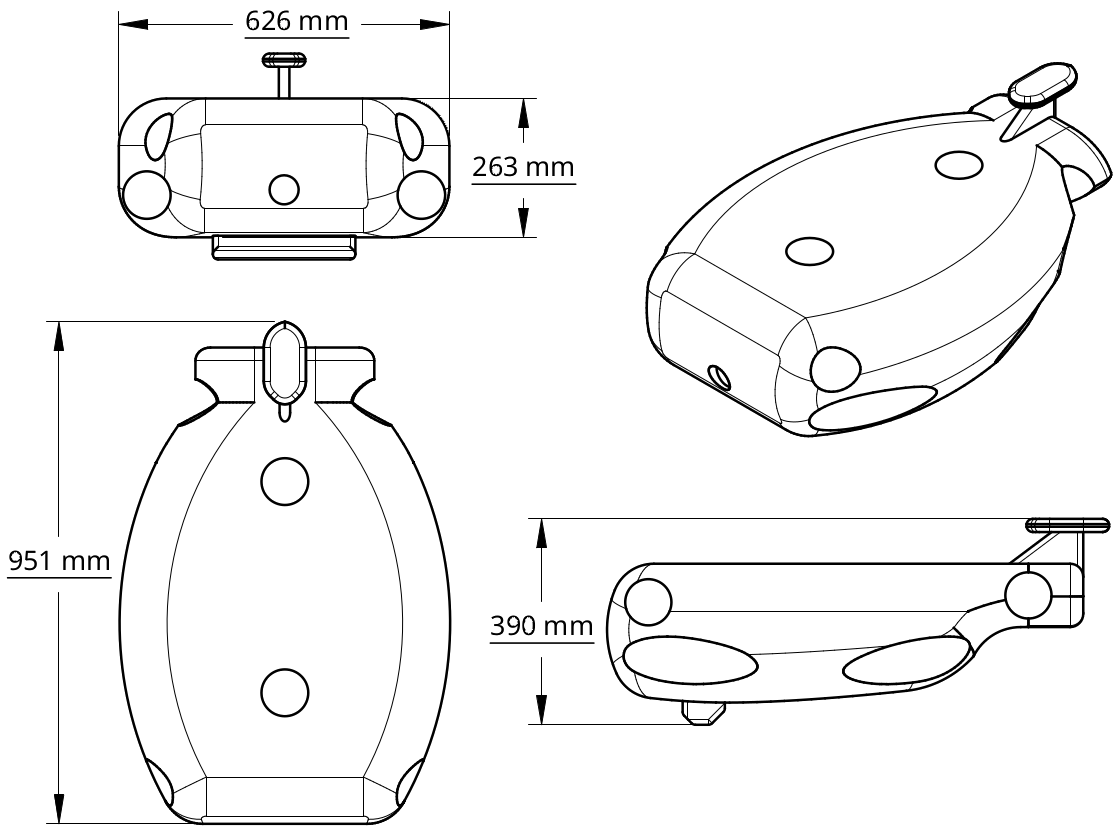
\includegraphics[width=.6\textwidth]{turbotplans.png}
  \end{center}
\end{frame}

%*----------- SLIDE -------------------------------------------------------------
\begin{frame}[c]{Sensors and peripherals}
  \transboxout[duration=0.5]
  Currently the turBOT project relies on these sensors, actuators and peripherals to perform the simulation:

  \begin{columns}
    \column{.02\textwidth}
    \column{.48\textwidth}
      \begin{enumerate}
        \item Low-light HD USB camera
        \item Minteye standard stereo camera
        \item Ping sonar altimeter and echosounder
        \item Red laser diode module
        \item MPU6050 IMU
        \item Venus638Flpx GPS
        \item Lumen Subsea Light
        \item Thruster Bluerobotics T200
      \end{enumerate}
    \column{.4\textwidth}
      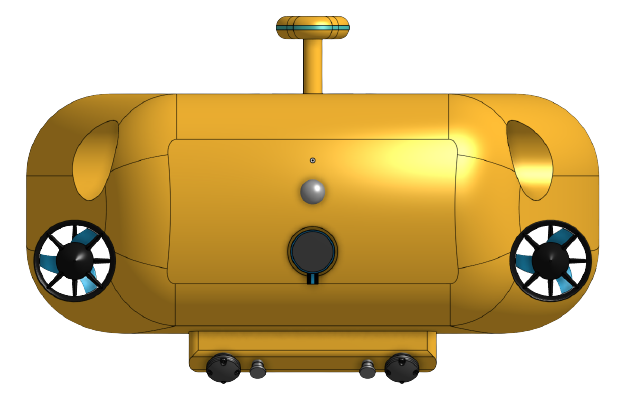
\includegraphics[width=1.0\textwidth]{turbot_front.png}      
  \end{columns}
\end{frame}

%*----------- SLIDE -------------------------------------------------------------
\begin{frame}[c]{Gazebo simulation}
  % \transboxout[duration=0.5]
  \centering
  \includemedia[
    width=.95\linewidth,
    totalheight=0.475\linewidth,
    activate=pageopen,
    passcontext, 
    addresource=Media/movies/turbot_video_cut.mp4,
    flashvars={
    source=Media/movies/turbot_video_cut.mp4
    &autoPlay=true
    &Loop=false}
    ]{\fbox{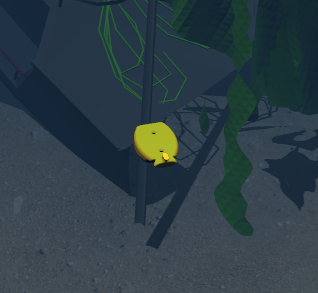
\includegraphics{turbot_intro}}}{VPlayer.swf}  
\end{frame}

